% ============================
% Extra 2
% ============================
%
\begin{tikzpicture}[x=1mm, y=1mm]
    \tikzmath{\fs = \textsize + 0.5;}
    
    % Parchment paper
    \draw[fill=parchment] (0,0) rectangle (63,88);
    
    % Imagem
    \node[anchor=north west, inner sep=0,outer sep=0] (image) at (0, 88) {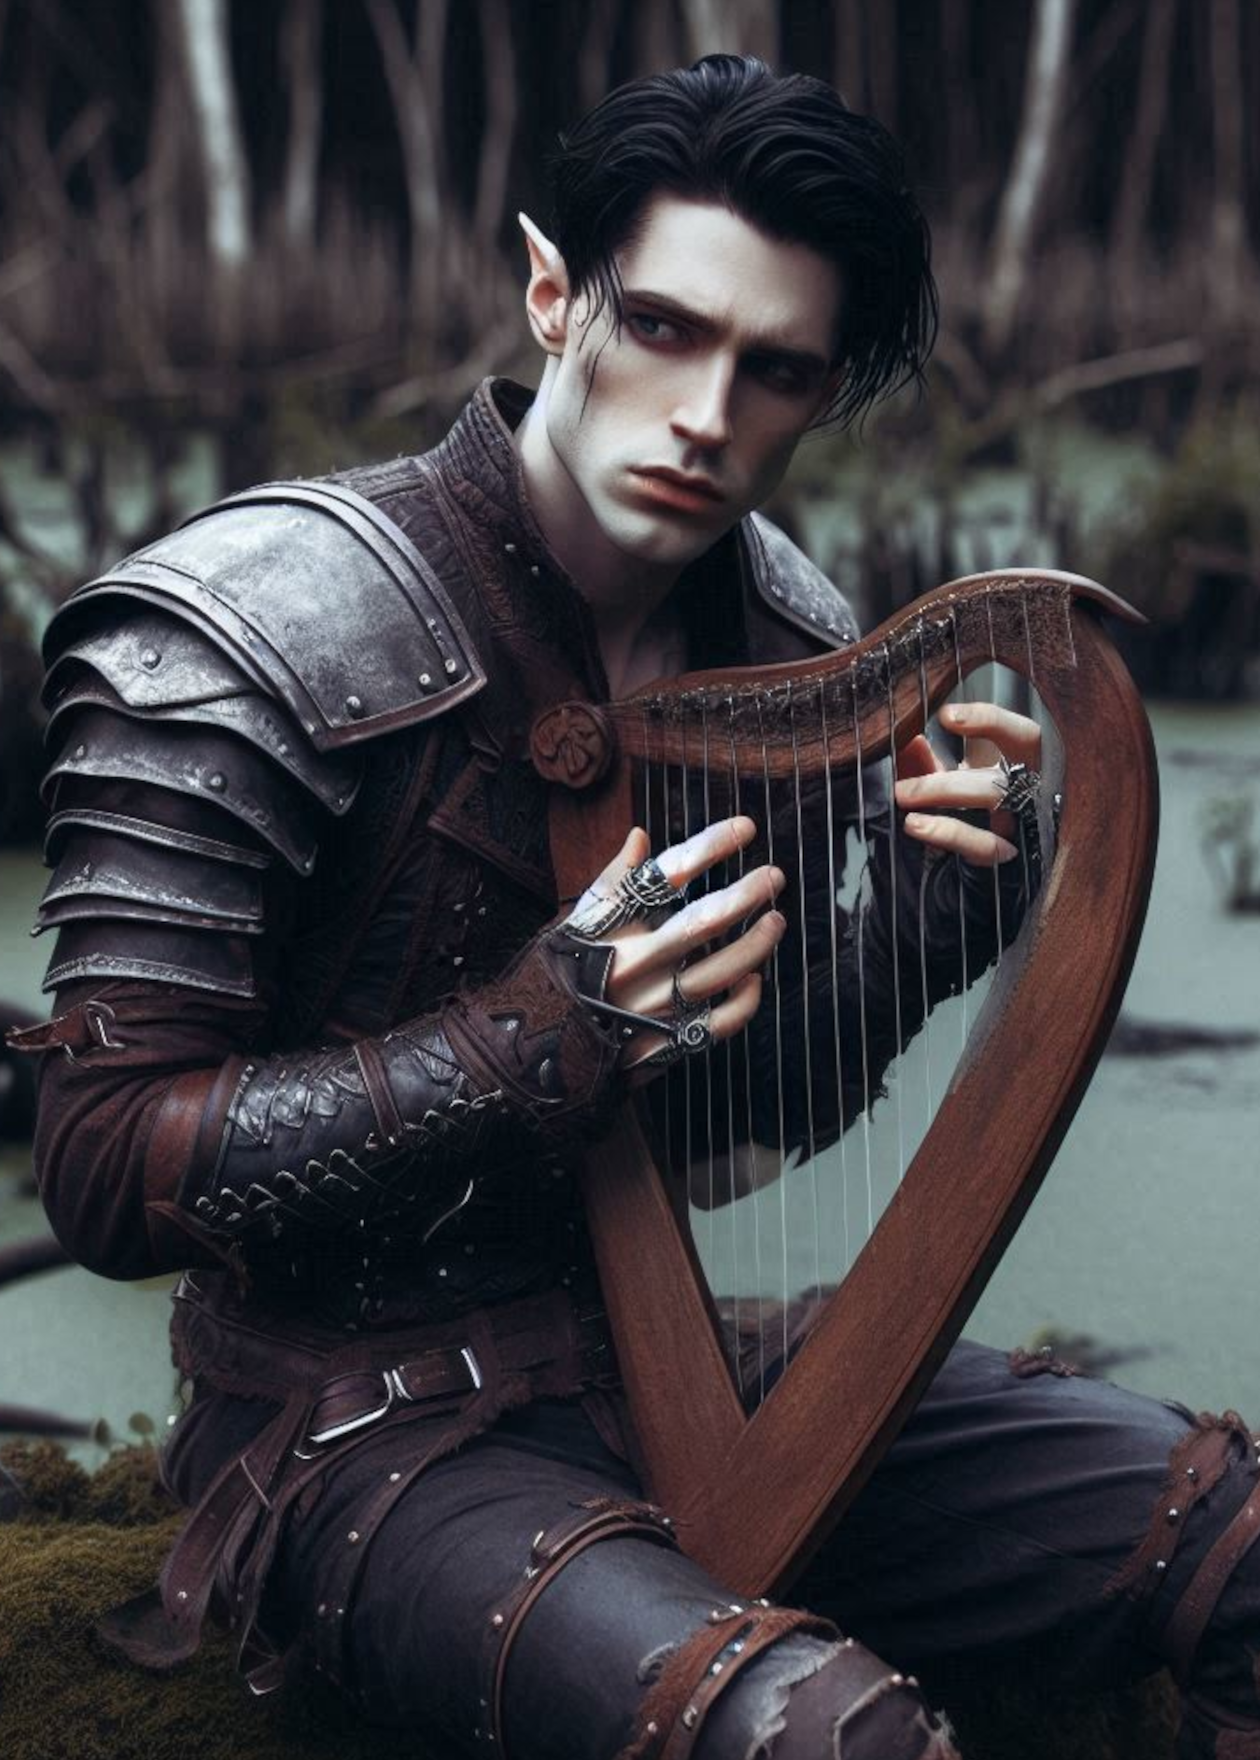
\includegraphics[width=63mm, height=88mm]{images/gon.png}};
    
    % Título
    \node[title, anchor=north west, minimum width=59mm](title) at (2,86) {Extra info of \textbf{Gon} - 2};
    

    % \textbf{Wild Shape:} The power of nature allows you to assume the form of an animal. As a Bonus Action, you shape-shift into a Beast form that you have learned for this feature.
    % You stay in that form for a number of hours equal to half your Druid level or until you use Wild Shape again, have the Incapacitated condition, or die. You can also leave the form
    % early as a Bonus Action.\\[0.5em]
    % \textbf{Rules While Shape-Shifted:} While in a form, you retain your personality, memories, and ability to speak, and the following rules apply:\\
    % \textbf{Temporary Hit Points:} \sout{When you assume a Wild Shape form, you gain a number of Temporary Hit Points equal to your Druid level.}\\
    % \textbf{Game Statistics:} Your game statistics are replaced by the Beast's stat block, but you retain your creature type; Hit Points; Hit Point Dice; Intelligence, Wisdom,
    % and Charisma scores; class features; languages; and feats. You also retain your skill and saving throw proficiencies and use your Proficiency Bonus for them,
    % in addition to gaining the proficiencies ofthe creature. Ifa skill or saving throw modifier in the Beast's stat block is higher than yours, use the one in the stat block.\\
    % \textbf{No Spellcasting:} You can't cast spells, but shape- shifting doesn't break your Concentration or oth- erwise interfere with a spell you've already cast.\\
    % \textbf{Objects:} Your ability to handle objects is deter- mined by the form's limbs rather than your own. In addition, you choose whether your equipment falls in your space,
    % merges into your new form, or is worn by it. Worn equipment functions as normal, but the DM decides whether it's practical for the new form to wear a piece of equipment based
    % on the creature's size and shape. Your equipment doesn't change size or shape to match the new form, and any equipment that the new form can't wear must either fall to the ground
    % or merge with the form. Equipment that merges with the form has no effect while you're in that form.

    % DRUID
    \node[fill=parchment, opacity=0.7, text opacity=1, draw opacity=1, inner sep=0mm, anchor=north west, font=\sffamily\fontsize{8}{8.5}, draw=black, rounded corners=0.4mm, fit={(2,80) (61,2)}] (WILDSHAPE) {};
    \node[tag, anchor=west] at ([xshift=0.5mm] WILDSHAPE.north west) {WILD SHAPE};
    \node[anchor=north west, align=justify, yshift=-1mm, text width=27mm, font=\sffamily\fontsize{4.5}{5}\selectfont] (wildshape) at (WILDSHAPE.north west) {%
    The power of nature allows you to assume the form of an animal. As a Bonus Action, you shape-shift into a Beast form that you have learned for this feature.
    You stay in that form for a number of hours equal to half your Druid level or until you use Wild Shape again, have the Incapacitated condition, or die. You can also leave the form
    early as a Bonus Action.\\[0.5em]
    \textbf{Challenge Rating:} The maximum Challenge Rating for the form equals your Druid level divided by 3 (round down).\\[0.5em]
    \textbf{Rules While Shape-Shifted:} While in a form, you retain your personality, memories, and ability to speak, and the following rules apply:\\[0.5em]
    %\textbf{Temporary Hit Points:} \sout{When you assume a Wild Shape form, you gain a number of Temporary Hit Points equal to your Druid level.}\\[0.5em]
    \textbf{Temporary Hit Points (Moon):} You gain a number of Temporary Hit Points equal to three times your Druid level.\\[0.5em]
    \textbf{Armor Class (Moon):} Until you leave the form, your AC equals 13 plus your Wisdom modifier if that total is higher than the Beast's AC.\\[0.5em]
    \textbf{Game Statistics:} Your game statistics are replaced by the Beast's stat block, but you retain your creature type; Hit Points; Hit Point Dice; Intelligence, Wisdom,
    and Charisma scores; class features; languages; and feats. You also retain your skill and saving throw proficiencies and use your Proficiency Bonus for them,
    in addition to gaining the proficiencies of the creature. If a skill or saving throw modifier in the Beast's stat block is higher than yours, use the one in the stat block.\\[0.5em]
    };
    
    \node[anchor=north west, align=justify, yshift=-1mm, text width=28mm, font=\sffamily\fontsize{4.5}{5}\selectfont] (wildshape) at ([xshift=28mm] WILDSHAPE.north west) {%
    \textbf{Limited Spellcasting (Moon):} You can't cast spells except for Circle of the Moon Spells (Cure Wounds, Moonbeam, Starry Wisp, Conjure Animals, ...). Shapeshifting doesn't
    break your Concentration or otherwise interfere with a spell you've already cast.\\[0.5em]
    \textbf{Objects:} Your ability to handle objects is determined by the form's limbs rather than your own. In addition, you choose whether your equipment falls in your space,
    merges into your new form, or is worn by it. Worn equipment functions as normal, but the DM decides whether it's practical for the new form to wear a piece of equipment based
    on the creature's size and shape. Your equipment doesn't change size or shape to match the new form, and any equipment that the new form can't wear must either fall to the ground
    or merge with the form. Equipment that merges with the form has no effect while you're in that form.\\[0.5em]
    };
    
    % EMPTY
    % \node[fill=parchment, opacity=0.7, text opacity=1, draw opacity=1, inner sep=0mm, anchor=north west, font=\sffamily\fontsize{8}{8.5}, draw=black, rounded corners=0.4mm, fit={(2,50) (61,2)}] (FIGHTER) {};
    % \node[tag, anchor=west] at ([xshift=0.5mm] FIGHTER.north west) {NOTES};

    % Borda
    \draw[line width = 0.5mm, black] (0,0) rectangle (63,88);
    
    \end{tikzpicture}%%